\documentclass[12pt]{article}
% This is for A4
% \usepackage[paperwidth=422mm, paperheight=303mm, left=3mm, right=3mm, top=3mm, bottom=3mm]{geometry}
% This is for B5
\usepackage[paperwidth=342mm, paperheight=246mm, left=3mm, right=3mm, top=3mm, bottom=3mm]{geometry}
\usepackage[absolute]{textpos}
\usepackage{charter} % new font
\usepackage{microtype}
\usepackage{tikz}
\usepackage{lmodern}
\setlength{\topskip}{0mm}
\setlength{\parindent}{0pt}
\setlength{\parskip}{0pt}
\usepackage{fancyhdr}
  \pagestyle{empty}
\usepackage{setspace}
  \setstretch{1.2}
\usepackage{xcolor}
  \definecolor{firebrick}{HTML}{B22222}
\begin{document}
\TPGrid{16}{16}\ttfamily

\begin{textblock}{7}[1,1](16,16)
  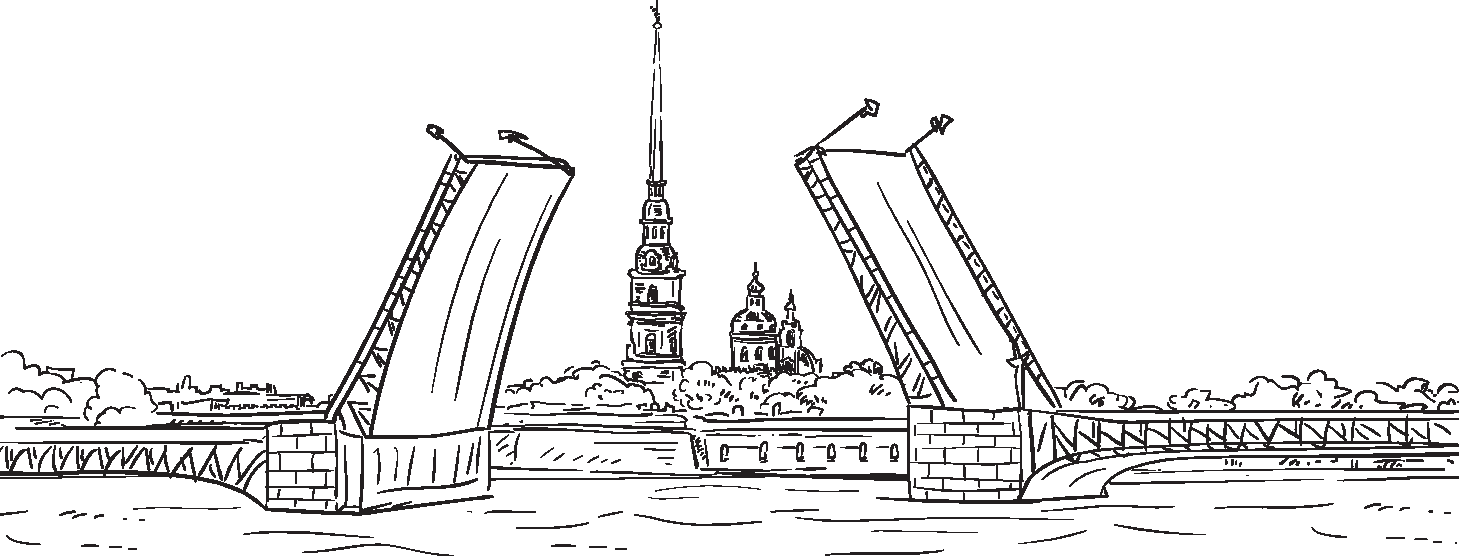
\includegraphics[width=7\TPHorizModule]{../../cfp/st-petersburg}
\end{textblock}

\begin{textblock}{2.4}[0.5,0](8,0)
  
\begin{tikzpicture}
    \node [rectangle, inner sep=0em, fill=firebrick, minimum width=2.4\TPHorizModule, minimum height=16\TPVertModule] at (0,0) {};
  \end{tikzpicture}
\end{textblock}

\begin{textblock}{7}[0,0](0,0)
  
\begin{tikzpicture}
    \node [rectangle, inner sep=0em, fill=firebrick, minimum width=7\TPHorizModule, minimum height=16\TPVertModule] at (0,0) {};
  \end{tikzpicture}
\end{textblock}

\begin{textblock}{1}[0.5,0](8,2)
  \begin{tikzpicture}
    \node [color=white, inner sep=0cm, outer sep=0cm, rotate=270, minimum height=\TPHorizModule] at (0,0) {
      \textbf{\large ICCQ'23}
    };
  \end{tikzpicture}
\end{textblock}

\begin{textblock}{1}[0.5,1](8,14)
  \begin{tikzpicture}
    \node [color=white, inner sep=0cm, outer sep=0cm, rotate=270, minimum height=\TPHorizModule] at (0,0) {
      \textbf{\large www.iccq.ru}
    };
  \end{tikzpicture}
\end{textblock}

\begin{textblock}{6}(10,4)
  \includegraphics[height=1.5in]{../../logo}
\end{textblock}

\begin{textblock}{6}(10,7)
  \fontsize{14}{14}\selectfont\textbf{%
    Proceedings of The Third \\
    International Conference on Code Quality \\
    April 2023, St. Petersburg, Russia
  }
\end{textblock}

\begin{textblock}{6}(10,9)
  \fontsize{12}{12}\selectfont\textbf{%
  Edited by Yegor Bugayenko and Andrey Terekhov}
\end{textblock}

\end{document}
